\section{DUNE Computing Model}
\label{sec:computing_model}

\subsection{Introduction}
The main purpose of the Computing Model is to guide the creation of DUNE computing fabric, spanning
hardware, middleware and various software components. Such fabric would give to all members of the DUNE
Collaboration unhindered access -- regardless of their location -- to reconstructed data for analysis, to various monitoring facilities,
to raw data for calibration and any other activities as required by the scientific objectives of the experiment. To meet these goals,
and in fulfillment of the data access requirements (\ref{sec:rules-of-access-to-data})
the model presented here has at  its core distributed data management and Grid and Cloud Computing concepts.

As stated in \ref{sec:modelrole}, the Computing Model is built on the basis of two supporting documents: the
``Software and Computing Requirements'', which sets forth policies and practices for the DUNE computing sector
(Sec.\ref{sec:requirements}), and ``DUNE Data Characteristics'' (Sec.\ref{sec:data-characteristics}) which contains information
necessary for quantifying parameters of the Computing Model.

\subsection{Data rate and volume estimates}

\subsubsection{Overview}
Rate and volume of the various data to be produced in DUNE are the major driver determining the parameters
of the Computing Model. Data types and their relationships were considered in Section~\ref{sec:data-characteristics},
and here a summary and aggregated estimates for the scale of the data will be presented.

\subsubsection{Raw Data}
Characteristics of the data to be produced by DUNE detector systems have been considered in
Sec.~\ref{sec:data-characteristics}.

At the time of writing estimations for the Far Detector data are better understood compared to other DUNE subsystems,
due to better developed geometry and parameters of the LArTPC, technology and configuration choices, and considerations
presented in subsections~\ref{sec:daq-assumptions},~\ref{sec:zs-data} and \ref{sec:data-compression}.

A distinguishing characteristic of the data flow in DUNE Far Detector is a significant data reduction factor to be achieved
in the Far Detector DAQ, as evidenced by the numbers presented in Tables~\ref{tab:full-stream-volume} and \ref{tab:zs-volume}.
The key assumption in this is the capability of DAQ to distinguish low energy signals  due to $^{39}$Ar decays spread
across the volume of the detector from more interesting physics phenomena (see~\ref{sec:ar39decays}).
This and similar capabilities will be provided
by deploying appropriate algorithms on the DAQ RCE and online farm utilizing about a hundred computers (estimated).
Estimates of volume of data due to high-energy interaction (cosmic $\mu$ and beam neutrinos) are presented in
Table~\ref{tab:fd-data-volume-summary} (page \pageref{tab:fd-data-volume-summary}) and are quite modest.

Processing required to identify candidate SNB and nucleon decay events will also be handled by the DAQ system and its online farm.
As discussed in subsection \ref{sec:snb-data}, once a SNB trigger condition has been established, the data must
be recorded without zero suppression in order to capture the characteristically low energy and scattered ionization
clusters in the detector volume as expected in a supernova burst event. As shown in Table~\ref{tab:zs-volume} (page~\pageref{tab:zs-volume}),
the resulting volume of data is significant and is currently estimated as just over half a PB annually, given the premise of accepting roughly
12 false positives per year. While the main goal of the SNB trigger is to provide a close to real-time Supernova Burst alert, the data
flagged by DAQ as candidate should not be discarded immediately even if near-time analysis indicated it was a false positive,
because such data can be used to better understand and improve online algorithms. For this reason it is assumed that
such data will be collected, transmitted and committed to storage.

Identifying candidate nucleon decay events will also require algorithms that would set the trigger condition consistent
with signatures such as $p \rightarrow K^+\nu$. As shown in \ref{sec:pdk-data}, the volume of data due to such candidate
events is not expected to be appreciable compared to other sources.

The Near Detector is quite different from the Far Detector in all of its characteristics, and it includes a number of subdetectors
such as Fine-Grained Tracker, Electromagnetic Calorimeter and others (see~\ref{sec:nds-event-rates}). There are a few technology
options being conisdered and most parameters are still being finalized at the time of writing, so data estimates are very preliminary.
It is conservatively assumed that the annual volume of these data will be 100\,TB.
%Current numbers result in annual volume from a few dozen to a hundred TB.

%In summary, it is anticipated that under assumptions presented above the total volume of data in DUNE to be
%committed to storage will be up to 1PB per year of data taking.

\subsubsection{Monte Carlo Data}
As discussed in \ref{sec:mc-data-estimates}, the Far and Near Detector simulation is the top contributor to the volume of overall
Monte Carlo in DUNE, with combined annual output of about 35\,TB of data. Other MC data sources are not appreciable.
It is reasonable to expect, that this number will grow as more effort becomes available for Monte Carlo studies and
as they become more sophisicated. However, at the time of writing there is no reliable estimate of how this segment of data
will scale over the years.


\subsection{Summary Table}

\subsection{Far Detector Data Handling}
\subsubsection{Conceptual Design of Data Flow}
A high-level conceptual diagram of the data flow in DUNE in presented in Fig.\ref{fig:DUNEdataflow}.
\begin{figure}[h!]
\centering
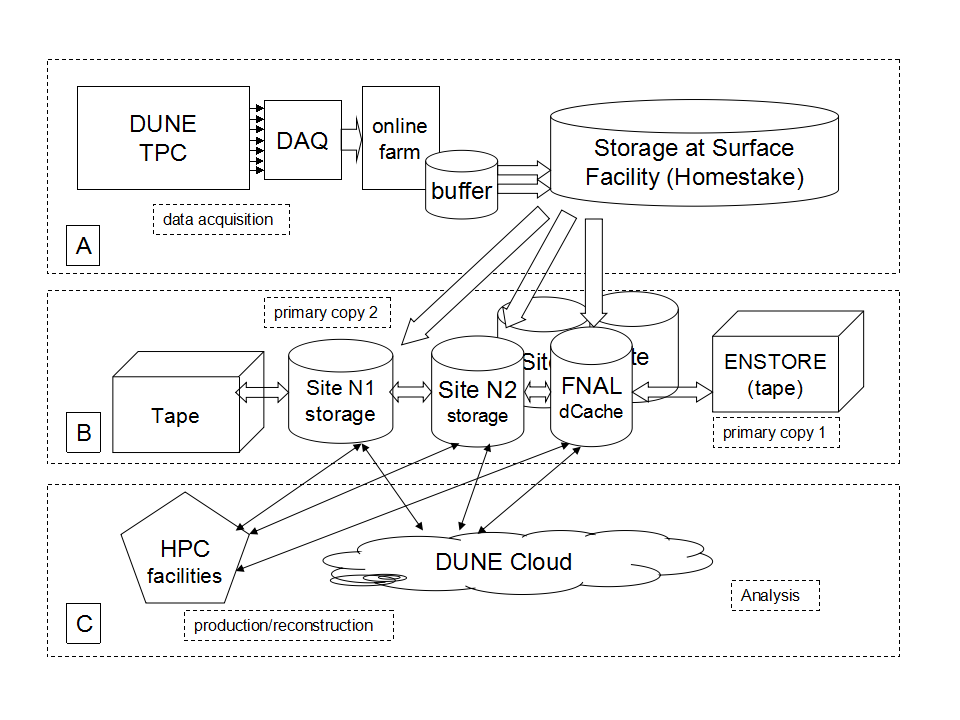
\includegraphics[width=\textwidth]{DUNEdataflow.png}
\caption{Conceptual Diagram of the Data Flow in DUNE.}
\label{fig:DUNEdataflow}
\end{figure}

\noindent
The top section of the diagram (labeled ``A'') represents systems and data flow at the Far Site.
The mid-section ``B'' depicts the DUNE data storage network. FNAL is the main data center
hosting tape storage for the primary copy of all data, as well as distributed disk (such as dCache).
It is expected that the Metadata system will also be deployed and operated at FNAL.
Additional Grid sites at participating institutions will have replicas of the data.
Replication of the data will be done as per requirements formulated in \ref{sec:req-raw-data-replication}.

\subsubsection{Data Buffering and Merging at the Far Site}
Data Acquisition systems will be located in the specially built rooms in the detector vicinity,
i.e. in the cavern deep underground (commonly referred to as 4850L). The undergound location is to be
connected to surface by 96-strand fiber optic cable, but this does not imply that all strands will be
utilized at any given time. The scale of bandwidth of an individual fiber is 10gbps. It can be therefore
expected that there will be ample headroom for data transmission to the surface under a variety of scenarios.

There will be two layers of data buffering: a buffer in DAQ before the data is transmitted to the surface,
and at the surface facility before the data is transmitted to FNAL which is the primary storage site and the
keeper of the custodial copy of the data.

It is a common practice to provide buffer space for the experiment which is sufficient for intermediate storage of data
for one or maybe a few days in order to keep running even in case of network equipment outages. Given the estimates
presented above, the decisive factor for determining the buffer size will be the data scale of candidate SNB events since
they are likely to be read out at full-stream rate (with lax or no zero-suppression) (see Table~\ref{tab:zs-volume}). The
size of each buffer (the online farm and the surface facility as drawn in section ``A'' of Fig.\ref{fig:DUNEdataflow})
can therefore be estimated as $\sim$50\,TB.

There are additional considerations due to the modular structure of the DUNE Far Detector
which is conceived as four individual TPC modules. In order have to have more flexibility and to minimize down time
and the number of potential single points of failure the DAQ will be segmented into four individual  systems each collecting
data from their respective module~(see \ref{sec:daq-architecture}). To ensure
consistency and simplicity of processing, it is desirable to merge the data streams coming from individual
detectors' DAQ systems at some point so that data is written to files contains readout for the full 4-module
DUNE detector. The surface facility is the optimal location for the merging to take place since it needs to be
equipped with storage and networking equipment for buffering purposes in any scenario.

\subsection{Data Handling at the Near Site}
\fxnote{Just a placeholder at this point}
The Near Site is located within the boundaries of Fermilab and therefore it is easier to provide networking and other services for data handling.

\subsection{DUNE Data Management}
\subsubsection{Evolution of Data Distribution at the LHC}

In formulating the architecture for data distribution in DUNE, it is helpful to study the experience of the LHC experiments,
since DUNE shares much of the same challenges: potentially significant  volume of data to be collected and processed,
projected long period of operation of the experiment, and geographically dispersed and diverse research communities joining the Collaboration.

When data management systems for the LHC experiments were designed and deployed around the turn of the century, it had to be done
against the backdrop of lack of universal access to high bandwidth networks across collaborations and/or substantial cost of such access~\cite{monarc},
along with reliability issues.
In order to maximize utilization of intellectual and technical resources spread around the globe, a model was adopted in which the computing resources
were organized as a hierarchy of Regional Centers, which allowed for tight control and optimization of data transmission. In this hierarchy, the following
levels were identified:
\begin{itemize}
\item Tier-0: CERN
\item Tier-1: National Center (large scale and expensive facility)
\item Tier-2: Regional Center (smaller, mostly for analysis, local center of expertise and maintenance)
\item Tier-3: Workgroup Servers at participating institutions
\item Tier-4: Individual computers (desktops)
\end{itemize}
\noindent
In this approach, distribution of data and access to it within an experiment is likewise hierarchical, as shown in Fig.\ref{fig:monarc}.
\begin{figure}[h!]
\centering
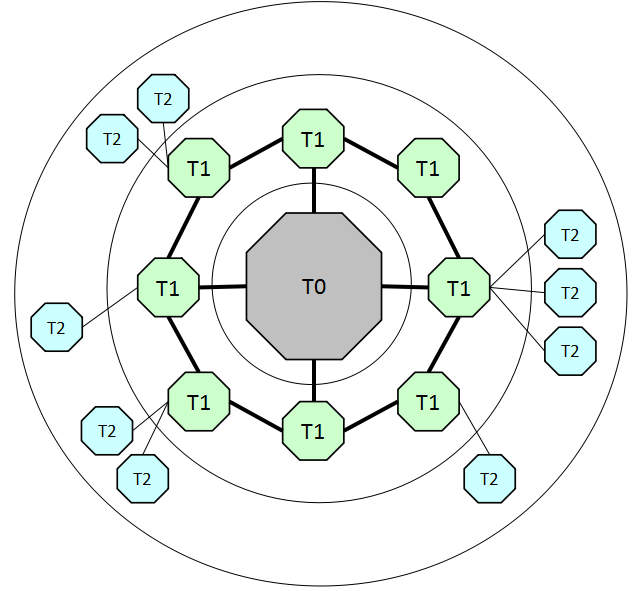
\includegraphics[width=0.6\textwidth]{monarc-model.png}
\caption{MONARC model of data distribution.}
\label{fig:monarc}
\end{figure}
Tier-1 centers have assured high bandwidth to CERN (Tier-0) and serve as the basis of further distribution of data
as required. Tier-2 centers would not be typically involved in large scale production activities and thus have reduced
network requirements. Smaller Tier-3 facilities would access data via Tier-2 etc.

We observe that at present, these experiments have actually revised the approaches to Data Handling and Workload
Management adopted in preparation for LHC Run-1~\cite{lhc_model_update}.
\begin{figure}[h!]
\centering
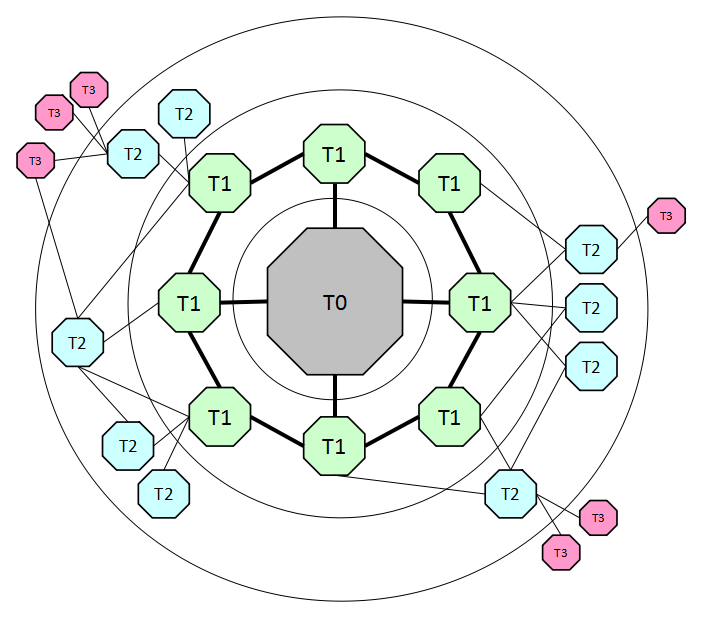
\includegraphics[width=0.6\textwidth]{un-monarc-model.png}
\caption{Evolved LHC model of data distribution.}
\label{fig:un-monarc}
\end{figure}
For Data Handling, there is a marked transition from the strictly hierarchical
“tiered” model of data distribution and access (e.g. MONARC) to more flat, agile, scalable and more peer-to-peer-like
architectures (see Fig.~\ref{fig:un-monarc}).
As stated in~\cite{lhc_model_update}
\begin{quotation}
\textit{With the technological progress of wide area networks and consequently improved network connectivity ATLAS has
already in Run-1 gradually moved away from the hierarchical association of Tier-2s to one Tier-1 (MONARC model)
and is now able to associate workflows between a well-connected Tier-2 and several Tier-1s, based on monitored
connectivity metrics. This functionality will be further pursued in Run-2 and is being incorporated into the production
system and distributed data management developments.}
\end{quotation}

\noindent
For Workload Management, there is more emphasis on access to heterogeneous and sometimes opportunistic resources, facilitated by dynamic software provisioning. Other challenges being addressed in LHC computing include the design and handling of Metadata, and managing computational workflows.


\subsubsection{Principles of Data Distribution}

\subsection{DUNE Analysis}
\subsubsection{Analysis Procedures and Data Flow}
\subsubsection{The Analysis Model}
\subsubsection{Distributed Analysis}

\subsection{Simulation}
\subsection{Calibration}
